\documentclass[11pt,a4paper]{article}
\usepackage[margin=2.3cm]{geometry}
\usepackage[T1]{fontenc}
\usepackage{mathptmx}
\renewcommand{\ttdefault}{pcr}
\usepackage{amsmath,amssymb}
\usepackage{booktabs,tabularx,array,multirow}
\usepackage{graphicx}
\usepackage{subcaption}
\usepackage{caption}
\usepackage{float}
\usepackage{enumitem}
\usepackage{xcolor}
\usepackage{tikz}
\usetikzlibrary{arrows.meta,positioning,calc,decorations.pathreplacing,shapes.geometric,fit,backgrounds}
\usepackage{algorithm}
\usepackage[noend]{algpseudocode}
\usepackage[hidelinks]{hyperref}
\usepackage[nameinlink]{cleveref}
\urlstyle{same}
\setlist{itemsep=2pt,topsep=4pt}
\captionsetup{font=small,labelfont=bf}
\renewcommand{\arraystretch}{1.2}
\newcolumntype{L}{>{\raggedright\arraybackslash}X}

\definecolor{male}{HTML}{3498DB}
\definecolor{maleD}{HTML}{1B4F72}
\definecolor{female}{HTML}{E91E63}
\definecolor{femaleD}{HTML}{880E4F}
\definecolor{keep}{HTML}{27AE60}
\definecolor{greedy}{HTML}{C0392B}
\definecolor{hot}{HTML}{E67E22}
\definecolor{grey}{HTML}{95A5A6}

\newcommand{\dirv}[1]{\mathbf{e}_{#1}}
\newcommand{\len}{\ell}
\newcommand{\Score}{\operatorname{score}}

\title{\textbf{The Family Metro Map Layout Algorithm}\\[2pt]
\large Design, beam search, scoring and overlap repair}
\author{Technical description of the implementation in \texttt{metro\_core.py}\\
(identical results to \texttt{familymetromap.js})}
\date{}

\begin{document}
\maketitle

\begin{abstract}
\noindent This document describes how the application draws a tree as an octilinear ``metro map'' in the style of Korst, Pronk and van Wijk (2020). The layout is built generation by generation: for every vertex, the directions, bends and lengths of the links to all of its children are chosen together by a small \emph{beam search} that scores every candidate by its conflicts, its clearance from the existing drawing, the free room it leaves for the child's own subtree, and metro-style preferences. Remaining vertex and edge overlaps are then detected and, on request, repaired by a budgeted local search. We define every quantity used by the code, walk through a real beam-search run step by step, analyse the running time, and report experiments on beam width and look-ahead, including cases where the beam search does \emph{not} help.
\end{abstract}

\setcounter{tocdepth}{1}
\tableofcontents
\bigskip

%==========================================================================
\section{Overview}

The input is an undirected tree $T=(V,E)$ with a chosen root $r$. Every vertex $v$ has a gender $\sigma(v)\in\{\mathrm F,\mathrm M\}$; in the application it is derived from the vertex label (the character code of its first letter is even for female). The output is a position $p_v\in\mathbb R^2$ for every vertex and, for some edges, one bend point. \Cref{fig:pipeline} shows the complete pipeline.

\begin{figure}[ht]
\centering
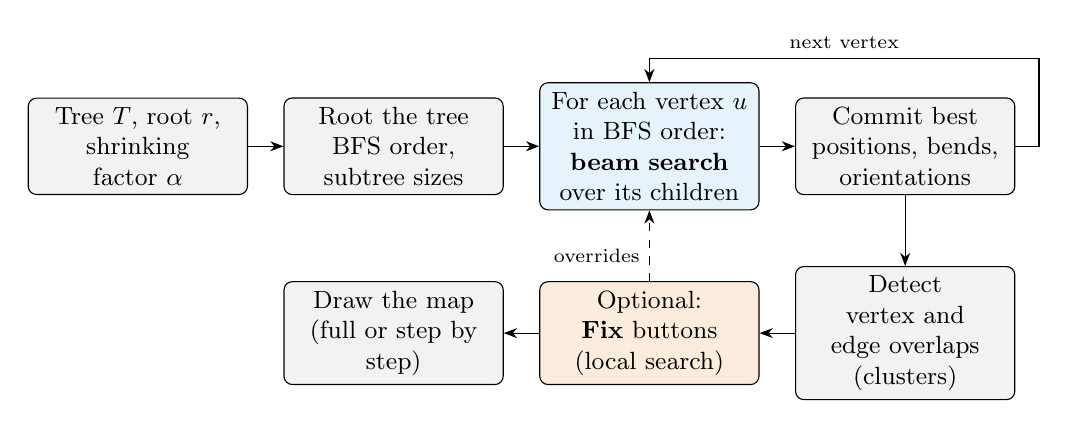
\begin{tikzpicture}[
  box/.style={draw, rounded corners=3pt, align=center, font=\small, minimum height=1.05cm, text width=2.55cm, fill=#1, execute at begin node=\hyphenpenalty 10000\relax},
  box/.default=white, >=Stealth, node distance=0.45cm]
\node[box=gray!10] (in) {Tree $T$, root $r$,\\ shrinking factor $\alpha$};
\node[box=gray!10, right=of in] (root) {Root the tree\\ BFS order,\\ subtree sizes};
\node[box=male!12, right=of root] (beam) {For each vertex $u$\\ in BFS order:\\ \textbf{beam search}\\ over its children};
\node[box=gray!10, right=of beam] (commit) {Commit best\\ positions, bends,\\ orientations};
\node[box=gray!10, below=0.9cm of commit] (detect) {Detect vertex and\\ edge overlaps\\ (clusters)};
\node[box=hot!15, left=of detect] (fix) {Optional:\\ \textbf{Fix} buttons\\ (local search)};
\node[box=gray!10, left=of fix] (draw) {Draw the map\\ (full or step by\\ step)};
\draw[->] (in) -- (root);
\draw[->] (root) -- (beam);
\draw[->] (beam) -- (commit);
\draw[->] (commit) -- (detect);
\draw[->] (detect) -- (fix);
\draw[->] (fix) -- (draw);
\draw[->, dashed] (fix.north) |- node[pos=0.25, left, font=\scriptsize]{overrides} ($(beam.south)+(0,-0.25)$) -- (beam.south);
\draw[->] (commit.east) -- ++(0.3,0) |- ($(beam.north)+(0,0.3)$) node[pos=0.75, above, font=\scriptsize]{next vertex} -- (beam.north);
\end{tikzpicture}
\caption{Pipeline. The layout (blue) is deterministic. The fixers (orange) do not move vertices directly; they record \emph{overrides} (forced choices for individual links) and re-run the layout.}
\label{fig:pipeline}
\end{figure}

The layout itself has four ingredients, each described in its own section:
\begin{enumerate}
  \item the \textbf{orientation and link model} (\cref{sec:links}): which directions a link may take and when it needs a bend;
  \item the \textbf{length model} (\cref{sec:length}): how long a link is, depending on its line generation;
  \item the \textbf{beam search} (\cref{sec:beam}): how the choices for all children of one vertex are made together;
  \item the \textbf{scoring function} (\cref{sec:score}): how one candidate placement is evaluated.
\end{enumerate}

%==========================================================================
\section{Orientation and link model}
\label{sec:links}

\subsection{Octilinear directions and gender}

All line segments are horizontal, vertical or diagonal. A direction is an integer $k\in\{0,\dots,7\}$ meaning the angle $k\cdot 45^\circ$, with unit vector
\[
  \dirv{k} = \bigl(\cos(k\pi/4),\ \sin(k\pi/4)\bigr).
\]
Because screen coordinates grow \emph{downwards}, $k=2$ points down and angles turn clockwise on screen (\cref{fig:compass}). Each vertex $v$ receives an \emph{orientation} $k(v)$: the direction of the last segment of the link that arrives at $v$. Following the paper, the orientation encodes gender:
\[
  k(v) \text{ is even} \iff \sigma(v)=\mathrm F \quad(\text{horizontal/vertical}),\qquad
  k(v) \text{ is odd} \iff \sigma(v)=\mathrm M \quad(\text{diagonal}).
\]
The root has no incoming link; it is given $k(r)=2$ if female and $k(r)=3$ if male.

\begin{figure}[ht]
\centering
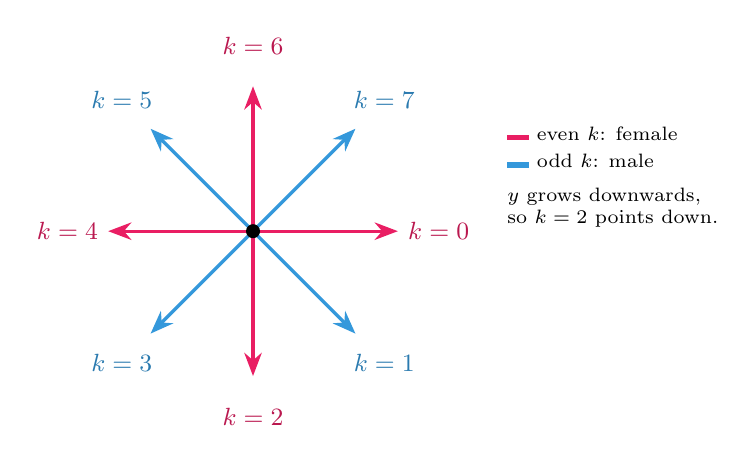
\begin{tikzpicture}[yscale=-1, >=Stealth, scale=1.15]
\foreach \k in {0,...,7} {
  \pgfmathsetmacro{\ang}{45*\k}
  \pgfmathtruncatemacro{\parity}{mod(\k,2)}
  \ifnum\parity=0 \def\col{female}\else\def\col{male}\fi
  \draw[->, very thick, \col] (0,0) -- (\ang:1.6);
  \node[font=\small, \col!80!black] at (\ang:2.05) {$k=\k$};
}
\fill[black] (0,0) circle (2.2pt);
\node[font=\scriptsize, align=left, anchor=west] at (2.7,-0.6) {\textcolor{female}{\rule{8pt}{2pt}} even $k$: female\\[2pt] \textcolor{male}{\rule{8pt}{2pt}} odd $k$: male\\[4pt] $y$ grows downwards,\\ so $k=2$ points down.};
\end{tikzpicture}
\caption{The eight octilinear directions. Even directions are used for female vertices and odd (diagonal) directions for male vertices.}
\label{fig:compass}
\end{figure}

\subsection{Branch offset $g$ and bend sign $s$}

Let $u$ be a vertex with orientation $k(u)$ and let $v$ be one of its children. The link $u\to v$ leaves $u$ with a \emph{first-segment direction}
\[
  d = \bigl(k(u)+g\bigr) \bmod 8, \qquad g\in\{0,\ +2,-2,\ +1,-1,\ +3,-3,\ 4\},
\]
where the \emph{branch offset} $g$ has the following meaning:

\begin{center}
\small
\begin{tabular}{@{}cll c@{}}
\toprule
$g$ & meaning & in the paper? & preference rank $\pi(g)$\\
\midrule
$0$ & continue the parent's metro line straight on & yes & 0\\
$\pm2$ & perpendicular T-junction (a new side line) & yes & 1\\
$\pm1$ & diagonal branch at $\pm45^\circ$ & no (high degree only) & 2\\
$\pm3$ & diagonal branch at $\pm135^\circ$ & no (high degree only) & 3\\
$4$ & opposite direction (only useful at the root) & no & 4\\
\bottomrule
\end{tabular}
\end{center}

The paper's family trees are binary (each person continues a line and starts at most one side line), so $g\in\{0,\pm2\}$ suffices there. A general tree can have up to seven children per non-root vertex, so the diagonal offsets are added as extra branch directions; their higher preference rank makes the search use them only when needed.

Whether the link needs a bend depends only on whether $d$ already has the right parity for $v$:
\[
  \text{straight link} \iff \bigl(d \text{ even}\bigr) = \bigl(\sigma(v)=\mathrm F\bigr), \qquad
  \text{otherwise a bended link with } s\in\{+1,-1\}.
\]
The final orientation is $k(v)=d$ for a straight link and $k(v)=(d+s)\bmod 8$ for a bended link, so the gender rule always holds.

\subsection{Link geometry}

For a link of (Euclidean) length $\len$:
\begin{align*}
  \text{straight:}\quad & p_v = p_u + \len\,\dirv{d},\\
  \text{bended:}\quad & b = p_u + \lambda\,\dirv{d},\qquad p_v = b + \lambda\,\dirv{d+s},\qquad \lambda = \frac{\len}{\sqrt{2+\sqrt2}} \approx 0.541\,\len .
\end{align*}
The value of $\lambda$ makes the distance $|p_v-p_u|$ exactly $\len$: the two segments of length $\lambda$ meet at an interior angle of $135^\circ$, so by the law of cosines $|p_v-p_u|^2 = 2\lambda^2(1-\cos 135^\circ) = \lambda^2(2+\sqrt2)=\len^2$. This is the construction of Section~4.1 of the paper. \Cref{fig:links} illustrates the three cases.

\begin{figure}[ht]
\centering
\begin{subfigure}[b]{0.28\textwidth}\centering
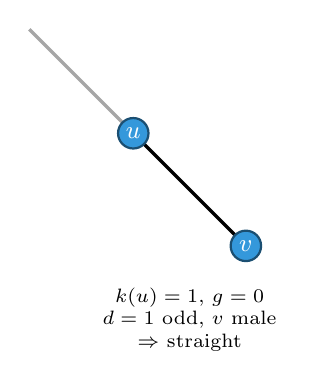
\begin{tikzpicture}[yscale=-1, scale=1.1, >=Stealth]
\draw[very thick, gray!70] (-1.2,-1.2) -- (0,0);
\draw[very thick] (0,0) -- (1.3,1.3);
\fill[male] (0,0) circle (5pt); \draw[maleD, thick] (0,0) circle (5pt);
\fill[male] (1.3,1.3) circle (5pt); \draw[maleD, thick] (1.3,1.3) circle (5pt);
\node[font=\small, white] at (0,0) {$u$}; \node[font=\small, white] at (1.3,1.3) {$v$};
\node[font=\scriptsize, align=center] at (0.65,2.15) {$k(u)=1$, $g=0$\\ $d=1$ odd, $v$ male\\ $\Rightarrow$ straight};
\end{tikzpicture}
\caption{straight link}\end{subfigure}
\hfill
\begin{subfigure}[b]{0.36\textwidth}\centering
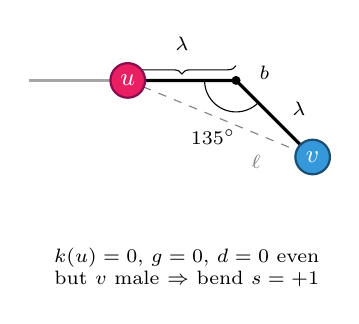
\begin{tikzpicture}[yscale=-1, scale=1.25, >=Stealth]
\coordinate (u) at (0,0); \coordinate (b) at (1.1,0); \coordinate (v) at ($(b)+(45:1.1)$);
\draw[very thick, gray!70] (-1.0,0) -- (u);
\draw[very thick] (u) -- (b) -- (v);
\draw[dashed, gray] (u) -- (v);
\node[font=\scriptsize, gray] at ($(u)!0.72!(v)+(-0.05,0.27)$) {$\len$};
\draw[decorate, decoration={brace, amplitude=3pt, mirror}] ($(u)+(0,-0.15)$) -- node[above=2pt, font=\scriptsize]{$\lambda$} ($(b)+(0,-0.15)$);
\node[font=\scriptsize] at ($(b)!0.5!(v)+(0.25,-0.1)$) {$\lambda$};
\draw (b) ++(180:0.32) arc (180:45:0.32);
\node[font=\scriptsize] at ($(b)+(112:0.62)$) {$135^\circ$};
\fill[female] (u) circle (5pt); \draw[femaleD, thick] (u) circle (5pt);
\fill[male] (v) circle (5pt); \draw[maleD, thick] (v) circle (5pt);
\node[font=\small, white] at (u) {$u$}; \node[font=\small, white] at (v) {$v$};
\fill (b) circle (1.3pt); \node[font=\scriptsize] at ($(b)+(-15:0.3)$) {$b$};
\node[font=\scriptsize, align=center] at (0.6,1.9) {$k(u)=0$, $g=0$, $d=0$ even\\ but $v$ male $\Rightarrow$ bend $s=+1$};
\end{tikzpicture}
\caption{bended link}\end{subfigure}
\hfill
\begin{subfigure}[b]{0.28\textwidth}\centering
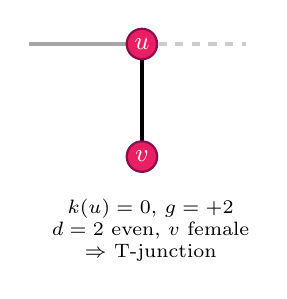
\begin{tikzpicture}[yscale=-1, scale=1.1, >=Stealth]
\draw[very thick, gray!70] (-1.3,0) -- (0,0);
\draw[very thick, gray!40, dashed] (0,0) -- (1.2,0);
\draw[very thick] (0,0) -- (0,1.3);
\fill[female] (0,0) circle (5pt); \draw[femaleD, thick] (0,0) circle (5pt);
\fill[female] (0,1.3) circle (5pt); \draw[femaleD, thick] (0,1.3) circle (5pt);
\node[font=\small, white] at (0,0) {$u$}; \node[font=\small, white] at (0,1.3) {$v$};
\node[font=\scriptsize, align=center] at (0.1,2.15) {$k(u)=0$, $g=+2$\\ $d=2$ even, $v$ female\\ $\Rightarrow$ T-junction};
\end{tikzpicture}
\caption{T-junction ($g=+2$)}\end{subfigure}
\caption{The three basic link types. Grey: the link arriving at $u$. The bended link has two segments of length $\lambda=\len/\sqrt{2+\sqrt2}$, so $v$ is still at distance $\len$ from $u$.}
\label{fig:links}
\end{figure}

\subsection{Distinct first directions}

A key rule, which removes most edge overlaps at their source, is that \emph{the links leaving a vertex use pairwise different first-segment directions}, and none of them uses the direction back along the incoming link, $(k(u)+4)\bmod 8$. Two links that start in the same direction would share their first segment, which the overlap detector reports as an edge overlap. A non-root vertex therefore has 7 free directions and the root 8; a vertex with more children than free directions cannot be drawn without an edge overlap, and only then is the rule relaxed (\cref{sec:beam}).

%==========================================================================
\section{Length model}
\label{sec:length}

The paper draws all links of a metro line of generation $g$ with the same length $\alpha^g$, where $0<\alpha\le 1$ is the shrinking factor: the root line has generation 0, its side lines generation 1, and so on. Here, the \emph{line generation} $\gamma(v)$ is defined along the tree:
\[
  \gamma(r)=0,\qquad
  \gamma(v)=\begin{cases}\gamma(u) & \text{if the link } u\to v \text{ continues the line } (g=0),\\ \gamma(u)+1 & \text{otherwise (a side line starts).}\end{cases}
\]
The length of the link $u\to v$ is
\[
  \len_{uv} = \max\Bigl(\ \max\bigl(L_0\,\alpha^{\gamma(v)},\ L_{\min}\bigr)\cdot f_{uv}\cdot \mu_u,\ \ L_{\text{abs}}\Bigr),
\]
with base length $L_0=90$\,px, floor $L_{\min}=34$\,px (so that the 16\,px vertex disks are always well apart), and a hard floor $L_{\text{abs}}=20$\,px. The factors $f_{uv}$ (length factor of one link) and $\mu_u$ (product of the local shrinking factors of all subtrees containing $u$) are $1$ unless the fixers have changed them (\cref{sec:fix}).

Note that the length depends on $g$ through $\gamma(v)$: continuing a line keeps the longer length of the parent's line, while a side line is shorter by a factor $\alpha$. This is one reason why continuing straight is often the cheapest option.

%==========================================================================
\section{Beam search over the children of one vertex}
\label{sec:beam}

\subsection{The decision problem at one vertex}

Vertices are processed in breadth-first order. When vertex $u$ is processed, $u$ itself and everything placed before it are fixed (``committed''). The task is to place all children $v_1,\dots,v_m$ of $u$, that is, to choose for each child an option
\[
  o_i = (g_i, s_i) \quad\Longrightarrow\quad d_i,\ \len_i,\ b_i,\ p_{v_i},\ k(v_i),
\]
such that the first directions $d_i$ are pairwise distinct and different from the back direction, and such that the total cost
\[
  \textstyle C(o_1,\dots,o_m) = \sum_{i=1}^{m} \Score\bigl(o_i \mid \text{committed geometry},\ o_1,\dots,o_{i-1}\bigr)
\]
is small. The score of a child depends on the siblings placed before it (they can collide with it), so the choices interact. With up to 12 options per child (8 offsets, half of them with two bend signs), exhaustive search costs up to $12^m$ evaluations, which is too many for vertices with many children. A purely greedy choice (best option for $v_1$, then best for $v_2$ given $v_1$, \dots) is cheap but may commit early to an option that leaves bad choices for later siblings. Beam search is the usual compromise between the two.

\subsection{Candidate options}

For each child $v$ the candidate list is built in a fixed order (this order also breaks ties):
\begin{enumerate}
  \item offsets $g$ in the order $0, +2, -2, +1, -1, +3, -3, 4$ (or only the forced offset if a fixer set one);
  \item for each offset: $s=0$ if the link is straight; otherwise $s=+1$ then $s=-1$ (or only the forced sign).
\end{enumerate}
With four even and four odd directions, exactly four offsets give straight links and four give bended links, so a child has $4+4\cdot2=12$ options. At a non-root vertex the offset $g=4$ is the blocked back direction, which leaves 10 or 11 usable options (as in \cref{tab:trace}, where J1 has 10). \Cref{fig:fan} shows the options around a vertex.

\begin{figure}[ht]
\centering
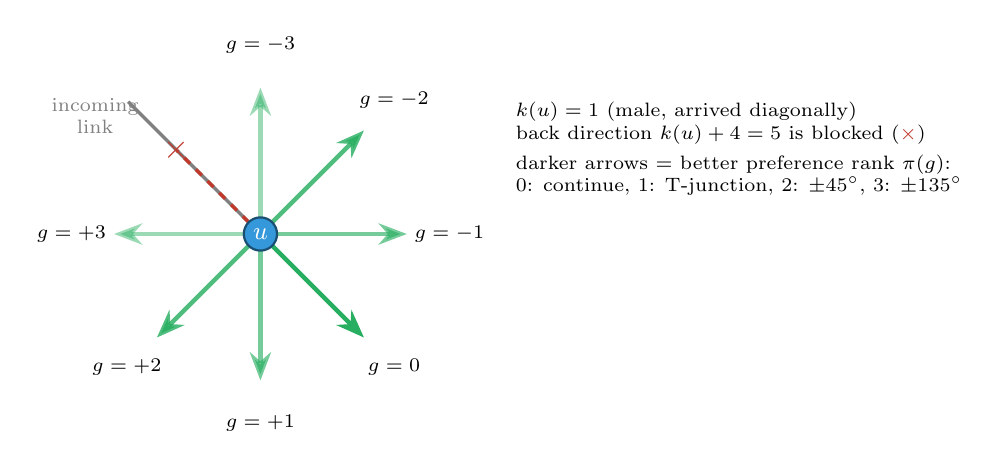
\begin{tikzpicture}[yscale=-1, scale=1.2, >=Stealth]
% incoming link along k(u)=1 (arrives travelling direction 1 = down-right)
\draw[very thick, gray] (-1.4,-1.4) -- (0,0);
\node[font=\scriptsize, gray, align=center] at (-1.75,-1.25) {incoming\\ link};
\foreach \g/\lab/\rk in {0/{$g=0$}/0, 2/{$g=+2$}/1, -2/{$g=-2$}/1, 1/{$g=+1$}/2, -1/{$g=-1$}/2, 3/{$g=+3$}/3, -3/{$g=-3$}/3} {
  \pgfmathsetmacro{\ang}{45*(1+\g)}
  \pgfmathsetmacro{\op}{1-0.18*\rk}
  \draw[->, line width=1.6pt, keep, opacity=\op] (0,0) -- (\ang:1.55);
  \node[font=\scriptsize] at (\ang:2.0) {\lab};
}
% blocked back direction k+4 = 5
\draw[line width=1.2pt, greedy, dashed] (0,0) -- (225:1.25);
\node[greedy, font=\large] at (225:1.25) {$\times$};
\fill[male] (0,0) circle (5pt); \draw[maleD, thick] (0,0) circle (5pt);
\node[white, font=\small] at (0,0) {$u$};
\node[font=\scriptsize, align=left, anchor=west] at (2.6,-0.9) {$k(u)=1$ (male, arrived diagonally)\\ back direction $k(u)+4=5$ is blocked (\textcolor{greedy}{$\times$})\\[3pt] darker arrows = better preference rank $\pi(g)$:\\ $0$: continue, $1$: T-junction, $2$: $\pm45^\circ$, $3$: $\pm135^\circ$};
\end{tikzpicture}
\caption{Candidate first directions at a non-root vertex. Each direction is used by at most one child. Whether a direction yields a straight or a bended link depends on the gender of the child.}
\label{fig:fan}
\end{figure}

\subsection{The beam}

A \emph{state} is a partial assignment $(o_1,\dots,o_j)$ for the first $j$ children together with its accumulated cost. The children are ordered by \emph{decreasing subtree size} (ties by their original order), so the largest subtrees choose first and get the best directions.

\begin{algorithm}[ht]
\caption{\textsc{PlaceChildren}$(u)$: beam search for the children of $u$ (beam width $B=4$)}
\label{alg:beam}
\begin{algorithmic}[1]
\State $v_1,\dots,v_m \gets$ children of $u$ sorted by subtree size (largest first)
\State $\mathit{blocked} \gets \{(k(u)+4)\bmod 8\}$ if $u\neq r$, else $\varnothing$
\State compute candidate options $O_i$ for every $v_i$ and the reach radius $R$ (\cref{sec:prune})
\State $\mathcal B \gets \{(\text{empty assignment},\ \text{cost } 0)\}$
\For{$i=1$ \textbf{to} $m$}
  \State $\mathcal N \gets \textsc{Expand}(\mathcal B, O_i, \text{distinct}=\textbf{true})$
  \If{$\mathcal N=\varnothing$} \Comment{more children than free directions, or forced choices clash}
     \State $\mathcal N \gets \textsc{Expand}(\mathcal B, O_i, \text{distinct}=\textbf{false})$
  \EndIf
  \State stable-sort $\mathcal N$ by cost; \ $\mathcal B \gets$ the first $B$ states of $\mathcal N$
\EndFor
\State commit the best state of $\mathcal B$: positions, bends, orientations $k(v_i)$, generations $\gamma(v_i)$
\Statex
\Function{Expand}{$\mathcal B, O, \text{distinct}$}
  \State $\mathcal N\gets\varnothing$
  \ForAll{states $S\in\mathcal B$}
    \State $\mathit{used}\gets \mathit{blocked}\ \cup$ \{first directions used in $S$\}
    \ForAll{options $o\in O$}
      \If{distinct \textbf{and} $d(o)\in\mathit{used}$} \textbf{continue} \EndIf
      \State compute $p_v$, $b$, $k(v)$ for $o$ \Comment{\cref{sec:links}}
      \State $c \gets \Score(o\mid \text{committed},\,S)$ \Comment{\cref{sec:score}}
      \State add $\bigl(S\cup\{o\},\ \mathrm{cost}(S)+c\bigr)$ to $\mathcal N$
    \EndFor
  \EndFor
  \State \Return $\mathcal N$
\EndFunction
\end{algorithmic}
\end{algorithm}

With $B=1$ this is exactly the greedy algorithm; with $B=\infty$ it is exhaustive search. Because the sort is stable and the option order is fixed, the result is deterministic: running the layout twice gives the same map, and the JavaScript and Python implementations produce identical coordinates.

\subsection{A worked example}

\Cref{tab:trace} shows a real run from the 100-vertex example tree ($\alpha=0.75$, root A). Vertex I1 (male, orientation $k=3$) has three children: J1 (female), Q1 and U2 (both male). Part of the neighbourhood is already crowded, so many options are penalised. The ``penalty'' column is the geometric part of the score (clearance and look-ahead, \cref{sec:score}); none of the listed options has a conflict.

\begin{table}[H]
\centering\small
\begin{tabular}{@{}c l c r r r r l@{}}
\toprule
rank & state (previous choices) $\to$ new option & $d$ & penalty & pref. & avg.\ term & cost & \\
\midrule
\multicolumn{8}{@{}l}{\textbf{Level 1: child J1} (10 candidates, keep 4)}\\
0 & $\varnothing \to$ J1: $g=0,\ s=+1$ & 3 & 0.0 & 0 & $-7.56$ & $-7.56$ & kept (greedy pick)\\
1 & $\varnothing \to$ J1: $g=+1$ & 4 & 0.0 & 24 & $-7.23$ & 16.77 & kept\\
2 & $\varnothing \to$ J1: $g=+2,\ s=-1$ & 5 & 68.2 & 12 & $-7.03$ & 73.14 & kept\\
3 & $\varnothing \to$ J1: $g=-1$ & 2 & 523.8 & 24 & $-7.35$ & 540.44 & kept\\
4 & $\varnothing \to$ J1: $g=0,\ s=-1$ & 3 & 719.2 & 0 & $-7.64$ & 711.60 & pruned\\
5 & $\varnothing \to$ J1: $g=-3$ & 0 & 1\,000\,803.8 & 36 & $-6.57$ & $\approx10^6$ & pruned (conflict)\\
\midrule
\multicolumn{8}{@{}l}{\textbf{Level 2: child Q1} (38 candidates, keep 4)}\\
0 & [J1 $d$=4] $\to$ Q1: $g=-1,\ s=+1$ & 2 & 0.0 & 24 & $-7.44$ & 33.33 & kept\\
1 & [J1 $d$=3] $\to$ Q1: $g=+1,\ s=+1$ & 4 & 68.2 & 24 & $-7.03$ & 77.58 & kept (greedy pick)\\
2 & [J1 $d$=5] $\to$ Q1: $g=-1,\ s=+1$ & 2 & 0.0 & 24 & $-7.44$ & 89.70 & kept\\
3 & [J1 $d$=5] $\to$ Q1: $g=0$ & 3 & 101.1 & 0 & $-7.65$ & 166.56 & kept\\
4 & [J1 $d$=5] $\to$ Q1: $g=+1,\ s=-1$ & 4 & 204.5 & 24 & $-7.37$ & 294.24 & pruned\\
\midrule
\multicolumn{8}{@{}l}{\textbf{Level 3: child U2} (32 candidates)}\\
0 & [J1 5, Q1 2] $\to$ U2: $g=+1,\ s=-1$ & 4 & 204.5 & 24 & $-7.37$ & \textbf{310.80} & \textbf{winner}\\
1 & [J1 4, Q1 2] $\to$ U2: $g=-3,\ s=-1$ & 0 & 380.8 & 36 & $-6.41$ & 443.69 & \\
2 & [J1 3, Q1 4] $\to$ U2: $g=-1,\ s=+1$ & 2 & 380.8 & 24 & $-7.44$ & 474.91 & greedy result\\
\bottomrule
\end{tabular}
\caption{Beam-search trace at vertex I1. ``pref.'' is $12\,\pi(g)$ and ``avg.\ term'' is $-0.02\times$ the average distance to the placed vertices. The cost of a state is the cost of its parent state plus the new option's score.}
\label{tab:trace}
\end{table}

The greedy algorithm would take the cheapest option for J1 (continue straight, $-7.56$), but this leaves Q1 and U2 only poor directions, ending at a total of 474.91. The beam keeps the third-best J1 option (73.14) alive; from it, Q1 and U2 find much better places and the total drops to 310.80. \Cref{fig:beamtree} draws the same search as a tree and \cref{fig:i1} shows the two resulting placements.

\begin{figure}[ht]
\centering
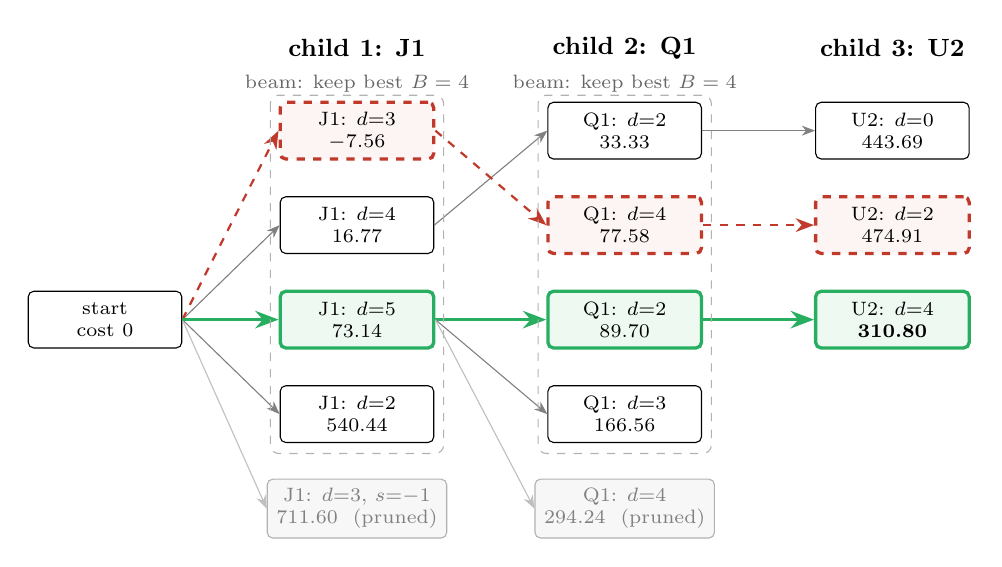
\begin{tikzpicture}[
  st/.style={draw, rounded corners=2pt, font=\scriptsize, align=center, minimum width=1.95cm, minimum height=0.72cm, fill=white},
  pruned/.style={st, draw=gray!60, text=gray, fill=gray!6},
  best/.style={st, draw=keep, very thick, fill=keep!8},
  grd/.style={st, draw=greedy, very thick, dashed, fill=greedy!5},
  >=Stealth, x=1cm, y=1cm]
\node[st] (r) at (0,0) {start\\ cost 0};
% level 1
\node[grd]  (a0) at (3.2, 2.4) {J1: $d$=3\\ $-7.56$};
\node[st]   (a1) at (3.2, 1.2) {J1: $d$=4\\ 16.77};
\node[best] (a2) at (3.2, 0.0) {J1: $d$=5\\ 73.14};
\node[st]   (a3) at (3.2,-1.2) {J1: $d$=2\\ 540.44};
\node[pruned] (a4) at (3.2,-2.4) {J1: $d$=3, $s$=$-1$\\ 711.60 \ (pruned)};
% level 2
\node[st]   (b0) at (6.6, 2.4) {Q1: $d$=2\\ 33.33};
\node[grd]  (b1) at (6.6, 1.2) {Q1: $d$=4\\ 77.58};
\node[best] (b2) at (6.6, 0.0) {Q1: $d$=2\\ 89.70};
\node[st]   (b3) at (6.6,-1.2) {Q1: $d$=3\\ 166.56};
\node[pruned] (b4) at (6.6,-2.4) {Q1: $d$=4\\ 294.24 \ (pruned)};
% level 3
\node[best] (c0) at (10.0, 0.0) {U2: $d$=4\\ \textbf{310.80}};
\node[st]   (c1) at (10.0, 2.4) {U2: $d$=0\\ 443.69};
\node[grd]  (c2) at (10.0, 1.2) {U2: $d$=2\\ 474.91};
% edges
\foreach \n in {a1,a3} \draw[->, gray] (r.east) -- (\n.west);
\draw[->, gray!50] (r.east) -- (a4.west);
\draw[->, greedy, thick, dashed] (r.east) -- (a0.west);
\draw[->, keep, very thick] (r.east) -- (a2.west);
\draw[->, gray] (a1.east) -- (b0.west);
\draw[->, greedy, thick, dashed] (a0.east) -- (b1.west);
\draw[->, keep, very thick] (a2.east) -- (b2.west);
\draw[->, gray] (a2.east) -- (b3.west);
\draw[->, gray!50] (a2.east) -- (b4.west);
\draw[->, keep, very thick] (b2.east) -- (c0.west);
\draw[->, gray] (b0.east) -- (c1.west);
\draw[->, greedy, thick, dashed] (b1.east) -- (c2.west);
% level labels
\node[font=\small\bfseries] at (3.2,3.45) {child 1: J1};
\node[font=\small\bfseries] at (6.6,3.45) {child 2: Q1};
\node[font=\small\bfseries] at (10.0,3.45) {child 3: U2};
\node[font=\scriptsize, gray!80!black] at (3.2,3.0) {beam: keep best $B=4$};
\node[font=\scriptsize, gray!80!black] at (6.6,3.0) {beam: keep best $B=4$};
\draw[gray!60, rounded corners=3pt, dashed] (2.1,2.85) rectangle (4.3,-1.7);
\draw[gray!60, rounded corners=3pt, dashed] (5.5,2.85) rectangle (7.7,-1.7);
\end{tikzpicture}
\caption{The beam search of \cref{tab:trace} (only a few of the expanded states are drawn). \textcolor{keep}{Green}: the path to the winning assignment. \textcolor{greedy}{Red, dashed}: the path greedy search ($B=1$) would follow. Grey boxes are pruned because they are not among the $B$ cheapest states of their level.}
\label{fig:beamtree}
\end{figure}

\begin{figure}[ht]
\centering
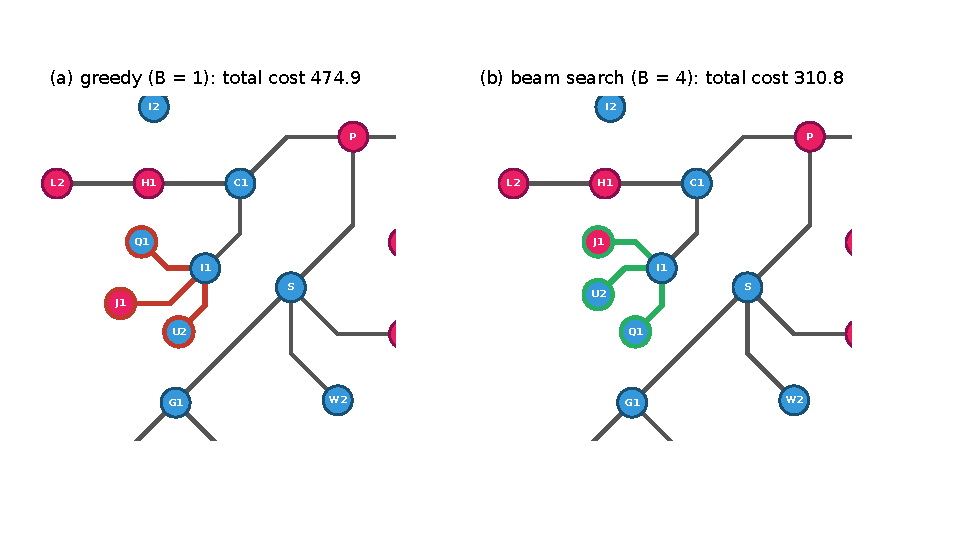
\includegraphics[width=0.92\textwidth]{fig_i1.pdf}
\caption{The two placements of I1's children from \cref{fig:beamtree}, drawn on top of the geometry that was committed before I1 was processed. Greedy (a) squeezes J1, Q1 and U2 against the existing lines; the beam (b) finds an arrangement with more clearance.}
\label{fig:i1}
\end{figure}

\subsection{Complexity}

Let $m_u$ be the number of children of $u$, $|O|\le 12$ the number of options per child, and $N_u$, $S_u$ the numbers of committed vertices and segments near $u$. Level $i$ expands at most $B$ states into at most $B\,|O|$ candidates, each scored in $O(N_u+S_u+i)$ time. Sorting adds $O(B|O|\log(B|O|))$ per level. The whole layout therefore costs
\[
  O\Bigl(\sum_u m_u\,B\,|O|\,(N_u+S_u)\Bigr) \;\subseteq\; O\bigl(B\,|O|\,n^2\bigr),
\]
because $\sum_u m_u=n-1$ and $N_u,S_u=O(n)$. The average-distance term (\cref{sec:score}) iterates over all placed vertices and is the only part that is always linear in $n$; the rest is limited to the neighbourhood of $u$. In practice the layout takes about 45\,ms for a 45-vertex tree and 0.1--0.2\,s for 100 vertices in Python (about 4--10 times less in JavaScript).

%==========================================================================
\section{The scoring function}
\label{sec:score}

\subsection{Definition}

Let $u$ be the parent, $o$ the option for child $v$ with resulting position $p_v$, optional bend $b$, final orientation $k(v)$ and length $\len$, and let $\Sigma_{\text{new}}$ be the one or two new segments. ``Existing'' means committed geometry near $u$ plus the tentative siblings of the current beam state. The score is
\[
  \Score(o) \;=\; 10^6\,V \;+\; 10^5\,E \;+\; 40\,\max(0,\ 0.9\len - c) \;+\; P_{\text{room}} \;+\; 12\,\pi(g) \;-\; 0.02\,\bar\delta,
\]
with the following terms (constants are summarised in \cref{tab:const}):

\begin{description}[leftmargin=1.2em, style=nextline]
\item[$V$ -- vertex conflicts] the number of
  (i) existing vertices $w\neq u$ with $|p_v-p_w|<26$\,px,
  (ii) pairs (existing vertex $w\neq u$, new segment) at distance $<12$\,px (a line running through a vertex), and
  (iii) existing segments at distance $<12$\,px from $p_v$ (the new vertex sits on a line).
\item[$E$ -- edge conflicts] the number of pairs (new segment, existing segment) for which the collision predicate of \cref{sec:collide} reports a crossing, a same-direction overlap, or a touch closer than 6\,px.
\item[$c$ -- clearance] $c=\min\bigl(\min_w |p_v-p_w|,\ \min_\sigma 1.5\cdot\mathrm{dist}(p_v,\sigma)\bigr)$ over existing vertices $w\neq u$ and existing segments $\sigma$ not incident to $u$; if nothing exists, $c=\len$. The penalty is only active below $0.9\len$, so it pushes vertices apart without forcing an ever-larger spread. This is the analogue of the paper's $c_1$ (minimum distance), extended to vertex--line distances, which the paper names as a weakness of $c_1$ alone.
\item[$P_{\text{room}}$ -- look-ahead] only if $v$ has children. Two sample points $q_t=p_v+t\,\len\,\dirv{k(v)}$ for $t\in\{0.6,\,1.2\}$ lie where $v$'s own line would continue. With $\rho$ the smallest distance from a sample point to an existing vertex ($\neq u$) or a segment not incident to $u$,
  \[ P_{\text{room}} = 15\, w_v\,\max(0,\ \len-\rho),\qquad w_v=\tfrac12\min(|T_v|-1,\,4), \]
  where $|T_v|$ is the size of $v$'s subtree. Bigger subtrees thus ask for more free space ahead.
\item[$12\,\pi(g)$ -- metro preference] continuing a line is free, a T-junction costs 12, diagonal branches 24 or 36.
\item[$\bar\delta$ -- spread] the average distance from $p_v$ to all placed vertices, a mild pull outwards; the analogue of the paper's $c_2$.
\end{description}

The weights are chosen so that the terms act roughly lexicographically: any conflict ($\ge 10^5$) outweighs every geometric penalty; the geometric penalties are typically tens to hundreds and therefore usually dominate the preferences (at most 48); and the spread term (a few units) mainly breaks near-ties. \Cref{fig:score} illustrates the geometric terms.

\begin{figure}[ht]
\centering
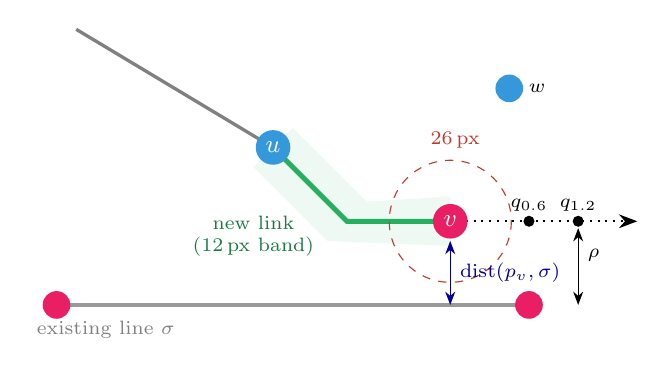
\begin{tikzpicture}[yscale=-1, scale=1.25, >=Stealth]
% existing geometry
\draw[very thick, gray!80] (-2.2,1.6) -- (2.6,1.6);
\fill[female] (-2.2,1.6) circle (4pt); \fill[female] (2.6,1.6) circle (4pt);
\fill[male] (2.4,-0.6) circle (4pt); \node[font=\scriptsize, right] at (2.5,-0.6) {$w$};
\node[font=\scriptsize, gray] at (-1.7,1.85) {existing line $\sigma$};
% u and incoming
\draw[very thick, gray] (-2.0,-1.2) -- (0,0);
\coordinate (u) at (0,0);
% new bended link
\coordinate (b) at (0.75,0.75); \coordinate (v) at (1.8,0.75);
\draw[line width=1.8pt, keep] (u) -- (b) -- (v);
% 12px band around new segments (schematic)
\fill[keep, opacity=0.08] ($(u)+(0.2,-0.2)$) -- ($(b)+(0.2,-0.2)$) -- ($(v)+(0,-0.25)$) -- ($(v)+(0,0.25)$) -- ($(b)+(-0.2,0.2)$) -- ($(u)+(-0.2,0.2)$) -- cycle;
% node clearance circle
\draw[dashed, greedy] (v) circle (0.62);
\node[font=\scriptsize, greedy] at ($(v)+(0.05,-0.82)$) {26\,px};
% look-ahead samples along k(v)=0 (right)
\draw[->, dotted, thick] (v) -- ++(1.9,0);
\fill (2.6,0.75) circle (1.6pt) node[above, font=\scriptsize] {$q_{0.6}$};
\fill (3.1,0.75) circle (1.6pt) node[above, font=\scriptsize] {$q_{1.2}$};
\draw[<->, thin] (3.1,0.82) -- (3.1,1.6) node[pos=0.35, right, font=\scriptsize] {$\rho$};
% distance to sigma
\draw[<->, thin, blue!60!black] (1.8,0.95) -- (1.8,1.6) node[midway, right, font=\scriptsize] {$\mathrm{dist}(p_v,\sigma)$};
\fill[male] (u) circle (5pt); \node[white, font=\small] at (u) {$u$};
\fill[female] (v) circle (5pt); \node[white, font=\small] at (v) {$v$};
\node[font=\scriptsize, keep!70!black, align=center] at (-0.2,0.9) {new link\\ (12\,px band)};
\end{tikzpicture}
\caption{Geometric quantities used by the score of a new link $u\to v$: the 26\,px vertex clearance circle, the 12\,px band around the new segments, the distance to a foreign line $\sigma$ (enters the clearance $c$ with factor 1.5), and the look-ahead samples $q_{0.6},q_{1.2}$ along $v$'s own direction with free room $\rho$.}
\label{fig:score}
\end{figure}

\begin{table}[ht]
\centering\small
\begin{tabular}{@{}l r l@{}}
\toprule
constant & value & role\\
\midrule
$L_0$ & 90\,px & base link length (root line)\\
$L_{\min}$, $L_{\text{abs}}$ & 34\,px, 20\,px & length floors (normal, after fixer shrinking)\\
vertex clearance & 26\,px & vertex--vertex conflict threshold in the score\\
line clearance & 12\,px & vertex--line conflict threshold in the score\\
edge tolerance & 6\,px & touching edges (score and overlap detection)\\
vertex overlap & 16\,px & two disks overlap (detection only)\\
$B$ & 4 & beam width\\
weights & $10^6$, $10^5$, 40, 15, 12, 0.02 & $V$, $E$, clearance, look-ahead, preference, spread\\
\bottomrule
\end{tabular}
\caption{Constants of the layout.}
\label{tab:const}
\end{table}

\subsection{Spatial pruning}
\label{sec:prune}

Before the beam search at $u$ starts, the committed vertices and segments are filtered to those within the reach radius $R=2.4\,\len_{\max}+36$\,px of $u$, where $\len_{\max}$ is the longest candidate link of any child. All new segments lie within $\len_{\max}$ of $u$, so every conflict threshold (26, 12 and 6\,px) and every clearance value below $0.9\len$ is unaffected by geometry outside $R$: those terms are computed exactly. The look-ahead samples reach up to $2.2\len$ from $u$, so for long links a far-away obstacle can be missed by $P_{\text{room}}$; the pruning is therefore a slight approximation of the look-ahead term only. The spread term $\bar\delta$ always uses all placed vertices.

\subsection{Relation to the paper's cost $C(M)$}

The paper compares complete maps lexicographically by $C(M)=(c_1,c_2)$: first the minimum distance between non-neighbouring vertices, then the average distance, and it treats crossings as a hard constraint. The score here is local (one link at a time, against the geometry known so far) and additive (so states of a beam can be compared by a single number). Crossings are a very large penalty instead of a hard constraint, so a drawing is always produced, even for trees that admit no crossing-free map.

%==========================================================================
\section{Collision predicate and overlap detection}
\label{sec:collide}

Two segments $[p_1,p_2]$ and $[p_3,p_4]$ belonging to different edges are tested as follows (\cref{fig:collide}):
\begin{enumerate}
  \item \textbf{Bounding boxes.} If the boxes are more than 6\,px apart, there is no collision (a pure speed-up).
  \item \textbf{Shared endpoint} (within 1\,px). The segments meet at a vertex or at a bend. They collide only if they leave the shared point in the same direction (angle difference $<0.05$\,rad); otherwise meeting is legitimate.
  \item \textbf{Proper crossing.} If no endpoint is shared and the orientation tests show that each segment separates the endpoints of the other, they cross (an \emph{overlap}).
  \item \textbf{Touch.} Otherwise, if one segment comes within 6\,px of the other (minimum of the four endpoint--segment distances), they \emph{touch}.
\end{enumerate}

\begin{figure}[ht]
\centering
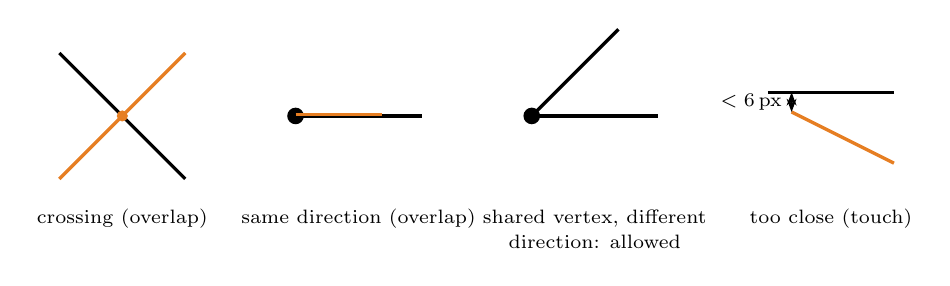
\begin{tikzpicture}[yscale=-1, scale=1.0, >=Stealth, every node/.style={font=\scriptsize}]
\begin{scope}
\draw[very thick] (0,0) -- (1.6,1.6); \draw[very thick, hot] (0,1.6) -- (1.6,0);
\fill[hot] (0.8,0.8) circle (2pt);
\node at (0.8,2.1) {crossing (overlap)};
\end{scope}
\begin{scope}[xshift=3cm]
\fill (0,0.8) circle (3pt);
\draw[very thick] (0,0.8) -- (1.6,0.8); \draw[very thick, hot] (0,0.78) -- (1.1,0.78);
\node at (0.8,2.1) {same direction (overlap)};
\end{scope}
\begin{scope}[xshift=6cm]
\fill (0,0.8) circle (3pt);
\draw[very thick] (0,0.8) -- (1.6,0.8); \draw[very thick] (0,0.8) -- (1.1,-0.3);
\node at (0.8,2.1) {shared vertex, different};
\node at (0.8,2.4) {direction: allowed};
\end{scope}
\begin{scope}[xshift=9cm]
\draw[very thick] (0,0.5) -- (1.6,0.5); \draw[very thick, hot] (0.3,0.75) -- (1.6,1.4);
\draw[<->, thin] (0.3,0.5) -- (0.3,0.75); \node[left] at (0.3,0.62) {$<6$\,px};
\node at (0.8,2.1) {too close (touch)};
\end{scope}
\end{tikzpicture}
\caption{Cases of the edge collision predicate.}
\label{fig:collide}
\end{figure}

After the layout, the overlap panels are computed on what is currently visible:
\begin{itemize}
  \item \textbf{Vertices:} the top-left pixel positions are rounded as on screen, and two vertices closer than 16\,px (the disk size) overlap.
  \item \textbf{Edges:} all pairs of drawn segments are tested with the predicate above.
\end{itemize}
In both cases the pairs are merged into connected components, so that three mutually overlapping vertices are reported once as ``Vertices B, H, N overlap''. During step-by-step drawing only vertices already drawn (and edges whose two endpoints are drawn) are checked, and components that did not exist in the previous step are marked NEW.

%==========================================================================
\section{Overlap repair (the Fix buttons)}
\label{sec:fix}

The layout is fast but local, so overlaps can remain, especially for small $\alpha$ or vertices of high degree. The two Fix buttons run a local search over \emph{overrides}, i.e.\ choices that the layout must respect:
\begin{itemize}
  \item a forced offset $g$ and/or bend sign $s$ for one link (the paper's suggestion of ``flipping'' subtrees, done automatically);
  \item a length factor $f_{uv}$ for one link;
  \item a local shrinking factor for the subtree below a vertex (a local version of Lemma 4.3 of the paper, which states that a small enough shrinking factor always separates neighbouring subtrees).
\end{itemize}
Because the layout is re-run after every change, everything placed after a modified link adapts automatically.

\begin{algorithm}[ht]
\caption{\textsc{Fix}$(\text{mode})$ with mode $\in\{\text{vertex},\text{edge}\}$}
\label{alg:fix}
\begin{algorithmic}[1]
\State $\mathit{best}\gets$ current overrides; \ $e\gets\textsc{Evaluate}(\mathit{best})$
\For{round $=1,\dots,16$ \textbf{while} overlaps of the chosen kind remain and budget is left}
  \State $\mathcal C\gets$ vertices involved in the overlaps, plus their parents and grandparents
  \ForAll{$x\in\mathcal C$ with parent $p$} \Comment{1. re-route one link}
     \ForAll{$(g,s)$ in the trial list of link $p\to x$}
        \State $e'\gets\textsc{Evaluate}(\mathit{best}+\{p\to x: g,s\})$
        \State remember it if $\mathrm{cost}(e')$ is the lowest so far (edge mode: and no new vertex overlaps)
     \EndFor
     \State accept the best trial for $x$ if it improves on the current cost
  \EndFor
  \If{nothing improved} try length factors $0.76$--$1.3$ for one link \Comment{2. rescale} \EndIf
  \If{nothing improved} try local shrinking $0.8, 0.65, 0.5$ for one subtree \Comment{3. Lemma 4.3} \EndIf
  \If{nothing improved} \textbf{stop} \EndIf
\EndFor
\State \Return $\mathit{best}$ and a summary of every accepted change
\end{algorithmic}
\end{algorithm}

\textsc{Evaluate} runs the full layout and computes
\begin{multline*}
  \mathrm{cost} = 100\,000\cdot(\#\text{vertex pairs closer than 16 px}) \\ + 5\,000\cdot(\#\text{colliding edge pairs}) - (\text{minimum vertex distance}).
\end{multline*}
The trial list for a link contains every offset $g\in\{\text{free},+2,-2,0,+1,-1,+3,-3\}$ (plus $4$ at the root), each with $s\in\{\text{free},+1,-1\}$ when the link is bended; variants that would not change anything are skipped. The search is deterministic and limited to $\max(150,\min(500,\lfloor25\,000/n\rceil))$ evaluations. \Cref{fig:fix21} shows its effect on a tree in which vertex C has eight children and therefore only seven free directions: one edge collision is unavoidable and is reported as unresolved.

\begin{figure}[ht]
\centering
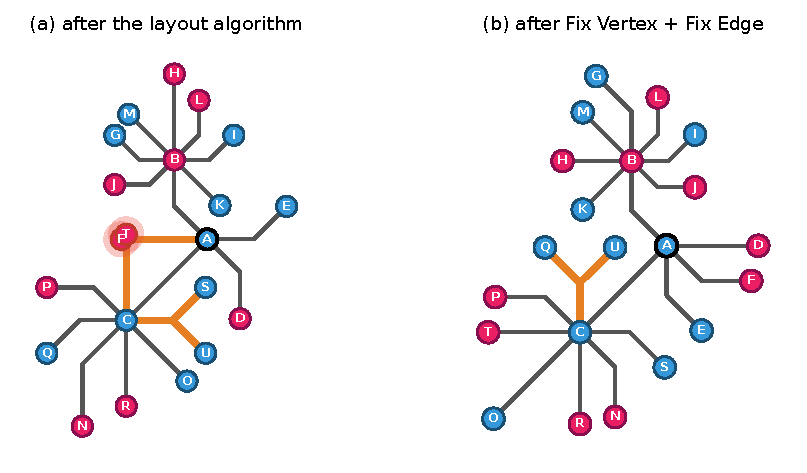
\includegraphics[width=0.85\textwidth]{fig_fix21.pdf}
\caption{A 21-vertex test tree ($\alpha=0.75$). (a) After the layout: vertices F and T overlap, and two groups of edges collide (orange). (b) After Fix Vertex Overlaps (``Relocated vertex F: branched as T-junction'') and Fix Edge Overlaps (two re-routed links): only C--Q and C--U still share their first segment, because C has more children than free directions.}
\label{fig:fix21}
\end{figure}

%==========================================================================
\section{Experiments}

\subsection{Effect of the design choices on overlaps}

The orientation model, distinct first directions and line generations were introduced to replace an earlier version that placed all children of a vertex relative to the same base direction and shrank every BFS level by $\alpha$. On 100 random trees with 10--45 vertices (at most 4 children per vertex), the total numbers of overlapping vertex pairs / colliding edge pairs after the layout alone were:

\begin{center}\small
\begin{tabular}{@{}l ccc@{}}
\toprule
 & $\alpha=1.0$ & $\alpha=0.75$ & $\alpha=0.5$\\
\midrule
earlier version & 540 / 725 & 508 / 737 & 3027 / 2661\\
current layout & 0 / 7 & 2 / 3 & 12 / 0\\
\bottomrule
\end{tabular}
\end{center}

\subsection{Beam width and look-ahead}

To see what the beam search and the look-ahead contribute, the layout was run with beam widths $B\in\{1,2,4,8\}$ and with the look-ahead term switched off, on three sets of random trees. \Cref{tab:beam} reports overlapping vertex pairs / colliding edge pairs (summed over the set) and, in brackets, the number of trees drawn without any overlap.

\begin{table}[ht]
\centering\footnotesize
\setlength{\tabcolsep}{4pt}
\begin{tabular}{@{}l c ccccc@{}}
\toprule
set & $\alpha$ & $B=1$ (greedy) & $B=2$ & $B=4$ (default) & $B=8$ & $B=4$, no look-ahead\\
\midrule
\multirow{2}{*}{\shortstack[l]{S: 100 trees,\\ 10--45 vertices}}
 & 1.0  & 0/2 (98) & 0/3 (99) & 0/5 (97) & 0/5 (96) & 0/5 (97)\\
 & 0.75 & 0/0 (100) & 0/0 (100) & 1/2 (98) & 2/2 (97) & 4/2 (96)\\
\midrule
\multirow{3}{*}{\shortstack[l]{L: 24 trees,\\ 60--100 vertices}}
 & 1.0  & 0/31 (7) & 0/40 (10) & 0/27 (12) & 0/45 (9) & 0/32 (11)\\
 & 0.75 & 4/2 (19) & 3/4 (20) & 21/9 (14) & 19/24 (13) & 30/47 (11)\\
 & 0.5  & 17/4 (15) & 19/6 (14) & 80/34 (4) & 76/28 (4) & 71/59 (3)\\
\midrule
\multirow{3}{*}{\shortstack[l]{H: 60 trees,\\ 30--60 vertices,\\ up to 6--8 children}}
 & 1.0  & 0/66 (35) & 0/44 (40) & 0/49 (38) & 0/49 (39) & 0/50 (34)\\
 & 0.75 & 3/15 (49) & 3/19 (50) & 23/21 (45) & 25/26 (43) & 26/40 (34)\\
 & 0.5  & 5/6 (52) & 11/9 (47) & 54/17 (45) & 73/42 (43) & 79/52 (31)\\
\bottomrule
\end{tabular}
\caption{Overlapping vertex pairs / colliding edge pairs after the layout (no fixers), and the number of overlap-free trees in brackets. Running time grows roughly linearly with $B$: per tree about 9, 13, 17, 28\,ms on set S and 95, 125, 190, 320\,ms on set L.}
\label{tab:beam}
\end{table}

\subsection{Discussion}

The results are mixed, and worth stating plainly:
\begin{itemize}
  \item The \textbf{look-ahead term helps} almost always: removing it from $B=4$ increases the number of collisions in almost every row, often substantially (e.g.\ 47 instead of 9 edge collisions on set L at $\alpha=0.75$).
  \item The \textbf{beam search optimises its local objective better} than greedy search (as in the example of \cref{tab:trace}), and at $\alpha=1$ it yields more overlap-free trees on the larger sets.
  \item However, for $\alpha\le0.75$ on large or dense trees, \textbf{greedy search ($B=1$) produced fewer overlaps} than the default $B=4$. Lower local cost does not always translate into a better final map: the summed score lets the search trade the free room of the largest subtree (placed first) for small gains such as preference points or spread of later siblings, and those trade-offs only show their consequences when the grandchildren are placed. Larger beams ($B=8$) do not fix this.
\end{itemize}
Possible improvements suggested by these findings are: comparing beam states lexicographically (conflicts, then clearance of the largest subtree first) instead of by a single sum; weighting the look-ahead more strongly for large subtrees; or simply running the layout with both $B=1$ and $B=4$ and keeping the map with the better global cost, which at most doubles the (small) layout time. The remaining overlaps are in any case handled by the Fix buttons.

%==========================================================================
\section{Differences from the paper and limitations}

\begin{itemize}
  \item The input is a general tree, not the paper's binary family tree with couples and age-ordered children; ``continuing a metro line'' is implicit ($g=0$).
  \item The paper's \emph{Clockwise} heuristic searches pairs of neighbouring lines in clockwise order with exhaustive sub-searches; here a per-vertex beam search in BFS order is used.
  \item Crossings are penalised rather than forbidden, and the cost is a weighted local score rather than the global lexicographic $C(M)$.
  \item The fixers may change single link lengths or shrink individual subtrees, which breaks the paper's equal spacing within a generation.
  \item The exhaustive (exact) search that the paper proposes for small trees is not implemented.
\end{itemize}

\begin{figure}[ht]
\centering
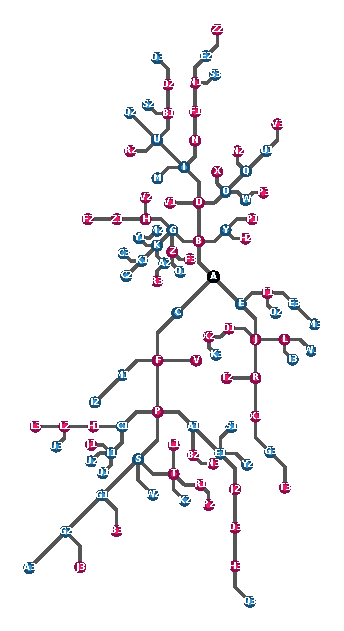
\includegraphics[width=0.8\textwidth]{fig_100.pdf}
\caption{The 100-vertex example tree drawn by the layout algorithm ($\alpha=0.75$, root A with black border), without any fixer; it has no vertex or edge overlaps.}
\label{fig:100}
\end{figure}

\vspace{1em}
\noindent\textbf{Reference.} J.~Korst, V.~Pronk and J.~J.~van Wijk. A Visualization of Family Relations Inspired by the London Metro Map. In \emph{The 13th International Symposium on Visual Information Communication and Interaction (VINCI 2020)}, Eindhoven, The Netherlands. ACM, 2020. \url{https://doi.org/10.1145/3430036.3430065}

\end{document}
